\documentclass[xcolor=x11names,compress]{beamer}
\usepackage[english]{babel}

%% General document %%%%%%%%%%%%%%%%%%%%%%%%%%%%%%%%%%

\usepackage{mathpazo}
\usepackage{graphicx}
\usepackage{tikz}
\usepackage{wrapfig}
\usepackage{hyperref}
\usepackage{fancybox,subcaption}
\usetikzlibrary{arrows}
\tikzstyle{block}=[draw opacity=0.7,line width=1.4cm]
\usetikzlibrary{decorations.fractals}
%%%%%%%%%%%%%%%%%%%%%%%%%%%%%%%%%%%%%%%%%%%%%%%%%%%%%%


%% Beamer Layout %%%%%%%%%%%%%%%%%%%%%%%%%%%%%%%%%%
\useoutertheme[subsection=false,shadow]{miniframes}
\useinnertheme{default}
\usefonttheme{serif}
\usepackage{palatino}

\setbeamerfont{title like}{shape=\scshape}
\setbeamerfont{frametitle}{shape=\scshape}

\setbeamercolor*{lower separation line head}{bg=DeepSkyBlue4} 
\setbeamercolor*{normal text}{fg=black,bg=white} 
\setbeamercolor*{alerted text}{fg=red} 
\setbeamercolor*{example text}{fg=black} 
\setbeamercolor*{structure}{fg=black}	%The color of title texts 
 
\setbeamercolor*{palette tertiary}{fg=black,bg=black!10} 
\setbeamercolor*{palette quaternary}{fg=black,bg=black!10} 


\newenvironment<>{problock}[1]{%
  \begin{actionenv}#2%
      \def\insertblocktitle{#1}%
      \par%
      \mode<presentation>{%
        \setbeamercolor{block title}{fg=white,bg=DeepSkyBlue4}
       \setbeamercolor{block body}{fg=black,bg=black!10}
       \setbeamercolor{itemize item}{fg=blue!20!black}
       \setbeamertemplate{itemize item}[triangle]
     }%
      \usebeamertemplate{block begin}}
    {\par\usebeamertemplate{block end}\end{actionenv}}


\useinnertheme[shadow=true]{rounded}
\usepackage{gnuplottex}
\renewcommand{\(}{\begin{columns}}
\renewcommand{\)}{\end{columns}}
\newcommand{\<}[1]{\begin{column}{#1}}
\renewcommand{\>}{\end{column}}
%%%%%%%%%%%%%%%%%%%%%%%%%%%%%%%%%%%%%%%%%%%%%%%%%%
\newcommand{\hlb}[1]{\textbf{\textcolor{DeepSkyBlue4}{#1}}}
\newcommand{\hl}[1]{\textcolor{blue}{#1}}
\newcommand{\lien}[2]{\mathcal{L}_{#1}^{#2}}
\newcommand{\lie}[1]{\mathcal{L}_{#1}}
\newcommand{\colv}[2]{\begin{pmatrix}#1\\#2\end{pmatrix}}
\newcommand{\colvt}[3]{\begin{pmatrix}#1\\#2\\#3\end{pmatrix}}
\newcommand{\bb}[1]{\textbf{#1}}
\newcommand{\mb}[1]{\mathbf{#1}}
\newcommand{\para}{\paragraph}
\newcommand{\subpara}{\subparagraph}
\newcommand{\abso}[1]{\left|#1\right|}


\usepackage[utf8]{inputenc}
%%%%%%%%%%%%%%%%% stuff for including svg images %%%%%%%%%%%%%
\newcommand{\executeiffilenewer}[3]{%
 \ifnum\pdfstrcmp{\pdffilemoddate{#1}}%
 {\pdffilemoddate{#2}}>0%
 {\immediate\write18{#3}}\fi%
}

\newcommand{\includesvg}[1]{%
 \executeiffilenewer{#1.svg}{#1.pdf}%
 {inkscape -z -D --file=#1.svg %
 --export-pdf=#1.pdf --export-latex}%
 \input{#1.pdf_tex}%
}








\begin{document}
\title{Investigating Piecewise Smooth Hybrid Systems}
\author{Debsankha Manik}

\begin{frame}
\titlepage
\end{frame}

\section{Introduction}
\begin{frame}{Hybrid systems}
These are systems described partly by differential equations and partly by 
maps: a \emph{hybrid} of continuous time and discrete time systems.  \\



\hlb{Examples:}
\begin{itemize}
\item A bell. 
\item A typewriter.  
\item Walking motion.  
\end{itemize}
\end{frame}

\begin{frame}{Hybrid Systems: Mathematical Definition}
\begin{problock}{definition}
A system described by a set of ODE's and a set of \bb{reset maps}:
\begin{align}
\label{def-hybrid}
\dot{x}&=F_i(x,\mu),~~\forall x\in S_i\\
x&\mapsto R_{ij}(x,\mu),~~\forall x\in\Sigma_{ij}=\bar{S_i}\cup\bar{S_j}
\end{align}

is called a piecewise smooth hybrid system if all the $R_i$'s, $F_i$'s as well 
as the associated flows $\varphi_i$'s are smooth in both $x$ and the parameter 
$\mu$ in the appropriate regimes.  
\end{problock}

\end{frame}


\begin{frame}{Example: Oscillator with hard impacts\\}
\begin{figure}[!hbp]
\caption{Hard impacting oscillator}
\label{fig-himp}
\begin{center}
\def\svgwidth{0.3\columnwidth}
\includesvg{hardcol}
\end{center}
\end{figure}

\begin{align}
\label{eq-hard_impact}
m\ddot{x}&=-\gamma \dot{x}-k_1x+G(t)&\mathrm{for}~~x<\sigma\\
(x,v)&\mapsto (x,-rv)&\mathrm{for}~~x=\sigma
\end{align}


$r$ is the coefficient of restitution, which is $1$ for perfectly 
elastic collisions.  
\end{frame}

\begin{frame}{Bifurcations in Hybrid Systems}
\hlb{Bifurcations} are \emph{qualitative} change in steady state system behaviour on a change of 
system parameters.  \\

\vspace{1em}
\pause{}
Bifurcations which are direct consequence of the switching  of the system dynamics
at the switching manifold are called \hlb{border collision bifurcations}.

\pause{}
\begin{tiny}
\begin{figure}
\begin{subfigure}{0.45\linewidth}
%\caption*{Before border collision: period 1}
\begin{center}
\def\svgwidth{0.9\linewidth}
\includesvg{pw-perdoub-bef}
\end{center}
\end{subfigure}%
$\to$
\begin{subfigure}{0.45\linewidth}
%\caption*{After border collision: period 2}
\begin{center}
\def\svgwidth{0.9\linewidth}
\includesvg{pw-perdoub-aft}
\end{center}
\end{subfigure}
\end{figure}
\end{tiny}
\end{frame}

\begin{frame}{Grazing bifurcation of limit cycles}
\begin{figure}[!htp]
\caption{Grazing orbit}
\label{fig-grazing-orbit}
\begin{center}
\def\svgwidth{0.7\columnwidth}
\includesvg{graz}
\end{center}
\end{figure}
\end{frame}

\section{The impact oscillator}
\begin{frame}
\begin{figure}[!hbp]
\caption{Hard impacting oscillator}
\label{fig-himp}
\begin{center}
\def\svgwidth{0.3\columnwidth}
\includesvg{hardcol}
\end{center}
\end{figure}

\begin{align}
\label{eq-hard_impact}
m\ddot{x}&=-\gamma \dot{x}-\omega_0^2x+F\cos{\omega 
t}&\mathrm{for}~~x<\sigma\\
(x,v)&\mapsto (x,-rv)&\mathrm{for}~~x=\sigma
\end{align}

\end{frame}


\begin{frame}{A few possible trajectories}

\begin{figure}
\begin{center}
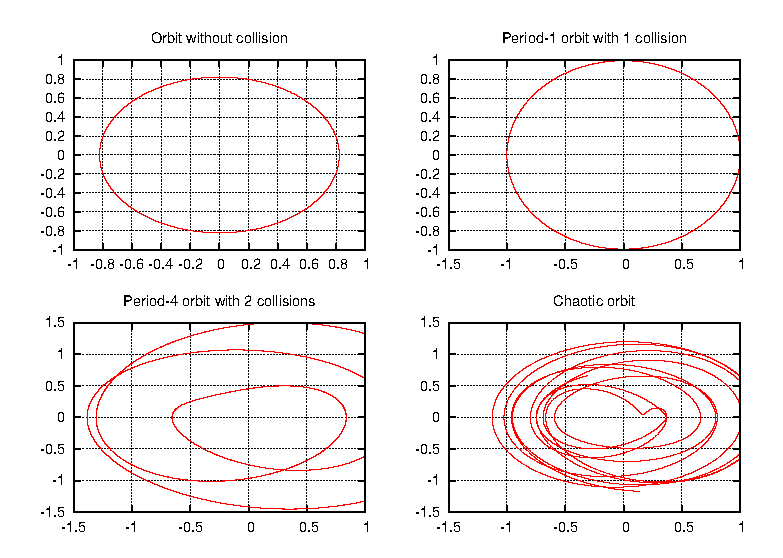
\includegraphics[width=\columnwidth]{many-orbs}
\end{center}
\end{figure}

\end{frame}

\begin{frame}{Stroboscopic Poincaré map}
\begin{figure}
\begin{center}
\def\svgwidth{0.9\columnwidth}
\includesvg{strobo}
\end{center}
\end{figure}
\end{frame}

\section{Vanishing Chaos}

\begin{frame}
Kundu and Banerjee \cite{banerjee-kundu-soft} investigated 
the grazing bifurcations in this system by deriving an approximate analytical expression 
for the stroboscopic  Poincaré map near grazing. \\


\hlb{Their results:}
\begin{itemize}
\item Unless $n=\frac{2\omega_g}{\omega_{forcing}}\in \mathbb{N}$, chaos \footnote{$\omega_g=\sqrt{\omega_0^2-\frac{\gamma^2}{4}}$}

immediately follows grazing of the steady state orbit.  
\item If $n\in\mathbb{N}$, no chaos after grazing.  
\end{itemize}
\hlb{Experimental data:}
\begin{itemize}
\item Chaos vanishes not only \emph{at} $n\in\mathbb{N}$, but at small 
neighbourhoods around each $n\in\mathbb{N}$
\end{itemize}
\end{frame}




















\end{document}
